\documentclass[12pt, titlepage]{article}
\usepackage{pifont}
\usepackage{booktabs}
\usepackage{tabularx}
\usepackage{pdfpages}
\usepackage{graphicx}
\usepackage{hyperref}
\usepackage{enumitem}
\usepackage{changepage}
\usepackage{tabto}
\usepackage{mdframed}
\usepackage{xkeyval}
\usepackage[round]{natbib}
\usepackage{soul}
\usepackage{color}

\hypersetup{
    colorlinks,
    citecolor=black,
    filecolor=black,
    linkcolor=red,
    urlcolor=blue
}
\usepackage[round]{natbib}
%% the following adds another section level by redefining the paragraph
%% source:  http://tex.stackexchange.com/questions/60209/how-to-add-an-extra-level-of-sections-with-headings-below-subsubsection
\setcounter{secnumdepth}{4}




%% Comments
\newif\ifcomments\commentstrue

\ifcomments
\newcommand{\authornote}[3]{\textcolor{#1}{[#3 ---#2]}}
\newcommand{\todo}[1]{\textcolor{red}{[TODO: #1]}}
\else
\newcommand{\authornote}[3]{}
\newcommand{\todo}[1]{}
\fi

\newcommand{\wss}[1]{\authornote{magenta}{SS}{#1}}
\newcommand{\ds}[1]{\authornote{blue}{DS}{#1}}



%% The following are used for pretty printing of events and requirements
\makeatletter

\define@cmdkey      [TP] {test}     {name}       {}
\define@cmdkey      [TP] {test}     {desc}       {}
\define@cmdkey      [TP] {test}     {type}       {}
\define@cmdkey      [TP] {test}     {init}       {}
\define@cmdkey      [TP] {test}     {input}      {}
\define@cmdkey      [TP] {test}     {output}     {}
\define@cmdkey      [TP] {test}     {pass}       {}
\define@cmdkey      [TP] {test}     {user}       {}


\newcommand{\getCurrentSectionNumber}{%
  \ifnum\c@section=0 %
  \thechapter
  \else
  \ifnum\c@subsection=0 %
  \thesection
  \else
  \ifnum\c@subsubsection=0 %
  \thesubsection
  \else
  \thesubsubsection
  \fi
  \fi
  \fi
}

\newcounter{TestNum}

\@addtoreset{TestNum}{section}
\@addtoreset{TestNum}{subsection}
\@addtoreset{TestNum}{subsubsection}

\newcommand{\testauto}[1]{
\setkeys[TP]{test}{#1}
\refstepcounter{TestNum}
\begin{mdframed}[linewidth=1pt]
\begin{tabularx}{\textwidth}{@{}p{3cm}X@{}}
{\bf Test \getCurrentSectionNumber.\theTestNum:} & {\bf \cmdTP@test@name}\\[\baselineskip]
{\bf Type:} & \cmdTP@test@type\\[0.5\baselineskip]
{\bf Initial State:} & \cmdTP@test@init\\[0.5\baselineskip]
{\bf Input:} & \cmdTP@test@input\\[0.5\baselineskip]
{\bf Output:} & \cmdTP@test@output\\[0.5\baselineskip]
{\bf Pass:} & \cmdTP@test@pass
\end{tabularx}
\end{mdframed}
}

\newcommand{\testautob}[1]{
\setkeys[TP]{test}{#1}
\refstepcounter{TestNum}
\begin{mdframed}[linewidth=1pt]
\begin{tabularx}{\textwidth}{@{}p{3cm}X@{}}
{\bf Test \getCurrentSectionNumber.\theTestNum:} & {\bf \cmdTP@test@name}\\[\baselineskip]
{\bf Description:} & \cmdTP@test@desc\\[0.5\baselineskip]
{\bf Type:} & \cmdTP@test@type\\[0.5\baselineskip]
{\bf Pass:} & \cmdTP@test@pass
\end{tabularx}
\end{mdframed}
}

\newcommand{\testmanual}[1]{
\setkeys[TP]{test}{#1}
\refstepcounter{TestNum}
\begin{mdframed}[linewidth=1pt]
\begin{tabularx}{\textwidth}{@{}p{3cm}X@{}}
{\bf Test \getCurrentSectionNumber.\theTestNum:} & {\bf \cmdTP@test@name}\\[\baselineskip]
{\bf Description:} & \cmdTP@test@desc\\[0.5\baselineskip]
{\bf Type:} & \cmdTP@test@type\\[0.5\baselineskip]
{\bf Tester(s):} & \cmdTP@test@user\\[0.5\baselineskip]
{\bf Pass:} & \cmdTP@test@pass
\end{tabularx}
\end{mdframed}
}


\makeatother

\title{\parbox{\linewidth}{\centering Test Report\endgraf\bigskip Super Tetris}}
\author{\parbox{\linewidth}{\bigskip \centering Group\#: 38 \endgraf\bigskip Team Name: Binary \endgraf\bigskip Members: \endgraf\bigskip Tongfei Wang : wangt62 \endgraf\bigskip Bowen Yuan : yuanb1 \endgraf\bigskip Tim Zhang : zhangj14}}
\date{\parbox{\linewidth}{\bigskip\bigskip \centering \today\endgraf\bigskip SFWR ENG 3XA3 \endgraf\bigskip McMaster University}}


\begin{document}

\maketitle

\pagenumbering{roman}
\tableofcontents
\listoftables
\listoffigures

\begin{table}[bp]
\caption{\bf Revision History}
\begin{tabularx}{\textwidth}{p{3cm}p{2cm}X}
\toprule {\bf Date} & {\bf Version} & {\bf Notes}\\
\midrule
Dec 6 2017& 1.0 & document upload\\
\bottomrule
\end{tabularx}
\end{table}

\newpage

\pagenumbering{arabic}


\section{Functional Requirements Evaluation}
\subsection{User Input and Navigation Test }


\testauto{
    name = {SP-IN1},
    type = {Functional,Dynamic,Manual},
    init =Web browser is open,
    input =  User enters the domain of this game,
    output = A new game starts,
    pass = Passed.
}

\testauto{
    name = {SP-IN2},
    type = {Functional,Dynamic,Manual},
    init =Game is in process,
    input =  User presses 'enter',
    output = Game paused,
    pass = Passed.
}


\testauto{
    name = {SP-IN3},
    type = {Functional,Dynamic,Manual},
    init =Game is paused,
    input =  User presses 'enter',
    output = Game resumes,
    pass = Passed.
}
					

\testauto{
    name = {SP-IN4},
    type = {Functional,Dynamic,Manual},
    init = Game is paused or in process,
    input =  User presses 'r',
    output = Game is restarted ,
    pass = Passed.
}


\testauto{
name = {SP-IN5},
type = {Functional,Dynamic,Manual},
init = Game is in process,
input =  User presses 'w',
output =  The current tetromino is rotated clockwise,
pass = Passed.
}

\testauto{
name = {SP-IN6},
type = {Functional,Dynamic,Manual},
init = Game is in process,
input =  User presses 'left' or 'right' by one grid,
output =  The current tetromino is moved left/right ,
pass = Passed.
}

\testauto{
name = {SP-IN7},
type = {Functional,Dynamic,Manual},
init = Game is in process,
input =  User presses 'down’,
output =  The current tetromino falls to the bottom(not intersected with other tetrominoes)  ,
pass = Passed.
}

\testauto{
name = {SP-IN8},
type = {Functional,Dynamic,Manual},
init = Game is in process,
input =  User presses '1' or '2' or '3' ,
output =  User buys and uses the item they selected('1' to  '3' correspanding to four different items), 
pass = Passed.
}



%%%%%%%%%%%%%%%%%%%%%%%%%%
\subsection{Game Logic Test}
~\newline

\testauto{
name = {SP-GL2},
type = {Structrual,Dynamic,Automated},
init = Game is in Process.,
input =  Coordinate of current tetromino which is a 4*4   matrix,
output =  True,
pass =  Passed
}

\testauto{
name = {SP-GL3},
type = {Structrual,Dynamic,Automated},
init = Game is in Process.,
input =  row number,
output =  new row ,
pass =  Passed.
}

\testauto{
name = {SP-GL4},
type = {Structrual,Dynamic,Automated},
init = Game is in Process.,
input =  N/A,
output =  A random 4*4 piece(tetromino),
pass = Passed.
}


\testauto{
name = {SP-GL7},
type = {Structrual,Dynamic,Automated},
init = Game is in Process.,
input =  item,
output =  True,
pass =  Passed.
}

\testauto{
name = {SP-GL9},
type = {Structrual,Dynamic,Automated},
init = Game is in Process.,
input =  Number of rows killed£¨playing time,
output =  Score increase 100 when one line is cleared,
pass =  Passed.
}

\testauto{
name = {SP-GL10},
type = {Structrual,Dynamic,Automated},
init = Game is in Process.,
input =  N/A,
output =  The speed of falling decrease for 15s,
pass =  Passed.
}

\testauto{
name = {SP-GL11},
type = {Structrual,Dynamic,Automated},
init = Game is in Process.,
input =  N/A,
output =  4*4  matrix  ,
pass =  Passed
}

\testauto{
name = {SP-GL12},
type = {Structrual,Dynamic,Automated},
init = Game is in Process.,
input =  N/A,
output =  Three rows are cleared,
pass =  Passed.
}

\testauto{
name = {SP-GL13},
type = {Structrual,Dynamic,Automated},
init = Game is in Process.,
input =  Playfield,
output =  True,
pass =  Passed.
}

\testauto{
name = {SP-GL14},
type = {Structrual,Dynamic,Automated},
init =State: Game is paused,
input =  N/A,
output =  No move happened,
pass =  Passed.
}

\section{Nonfunctional Requirements Evaluation}

\subsection{Usability}
		
\testmanual{
    name = Operating System Support,
    desc = Super Tetris shall run on all major web browsers ( Chrome/Firefox/Safari /IE) ,
    type = {Functional (dynamic, manual)},
    user = Development team,
    pass = {We run and play the game through Chrome/Firefox/Safari /IE successfully.}
}				

\testmanual{
    name = Look and Feel,
    desc = The falling of the tetrimino and line clear requires animation,
    type = {Functional (dynamic, manual)},
    user = Development team,
    pass = {When tetriminos are falling or when a row is eliminated, the animation display correctly. After we run the game hundreds of times we did not capture any incorrect animation display.}
}		

\testmanual{
    name = Difficulty,
    desc = Super Tetris shall follow the same rule in the Classic Tetris. ,
    type = {Functional (dynamic, manual)},
    user = Development team,
    pass = {Average survey score of less than 4 in 'Difficulty' section. The average survey score in Difficulty section amony the surveys we received are less than 4.  }
}		

\subsection{Performance}

\testmanual{
    name = Precision,
    desc =The event shall happen at the correct time. ,
    type = {Functional (dynamic, manual)},
    user = Development team,
    pass = {The boom shall explode when it stops. The ice shall slow the falling time when it is triggered. The line shall be cleared when a complete line is made. They are all triggered at the right timing.}
}
	
\testmanual{
    name = Capacity,
    desc = Super Tetris needs less than 10MB in memory. ,
    type = {Functional (dynamic, manual)},
    user = Development team,
    pass = {Test team calculates the size of whole program file before uploading. The whole game file takes less than 2MB in memory}
}

\subsection{Robustness}
\tab If an unexpected error occurs, the system will stop running at the first time. Additionally, The system is published on a server. The server we bought is robust and it will check if the system is cracked or a dead loop is running. If it is, the server will shut the system down and notice us.
	
\section{Comparison to Existing Implementation}	

\tab By comparing to the original implementation, this system makes several improvements. First, this system has a module structure which results in several modules while the original one has only one module. Secondly, we make the system connect to the server by coding some parts in HTML. Then, numerous functions and systems are added. Finally, our codes are well-commented while the existing code does not have any comment.



\section{Unit Testing}
\tab As the system is implemented by Javascript, Mocha was used for unit testing. The test coverts most of the functions and it called 'supertetristest.js' and can be found in 'src/mochatest/test'.
\section{Changes Due to Testing}
\tab While testing, we found that when a user uses the item “clear random three lines” the money was increased as three normal lines were eliminated. However, we planed the item costs $20 and the user gain $10 if a line is cleared. As a result, every time the user used this item, the user’s money will not decreased. In the contrary, the user gain $10 every time s/he used the item. For solving this problem, we increased the cost of this item to $100.

\section{Automated Testing}
\tab For Automated Testing, we used mocha unit test. For almost every function, it generates numerous inputs and check if the answers match the outputs and report them as “pass” or “fail”. Then it will classify where the issue comes from and what the supposed output is to make is traceable.	
\section{Trace to Requirements}
refer to the table in the end of the document.
\begin{figure}[h]
\centering
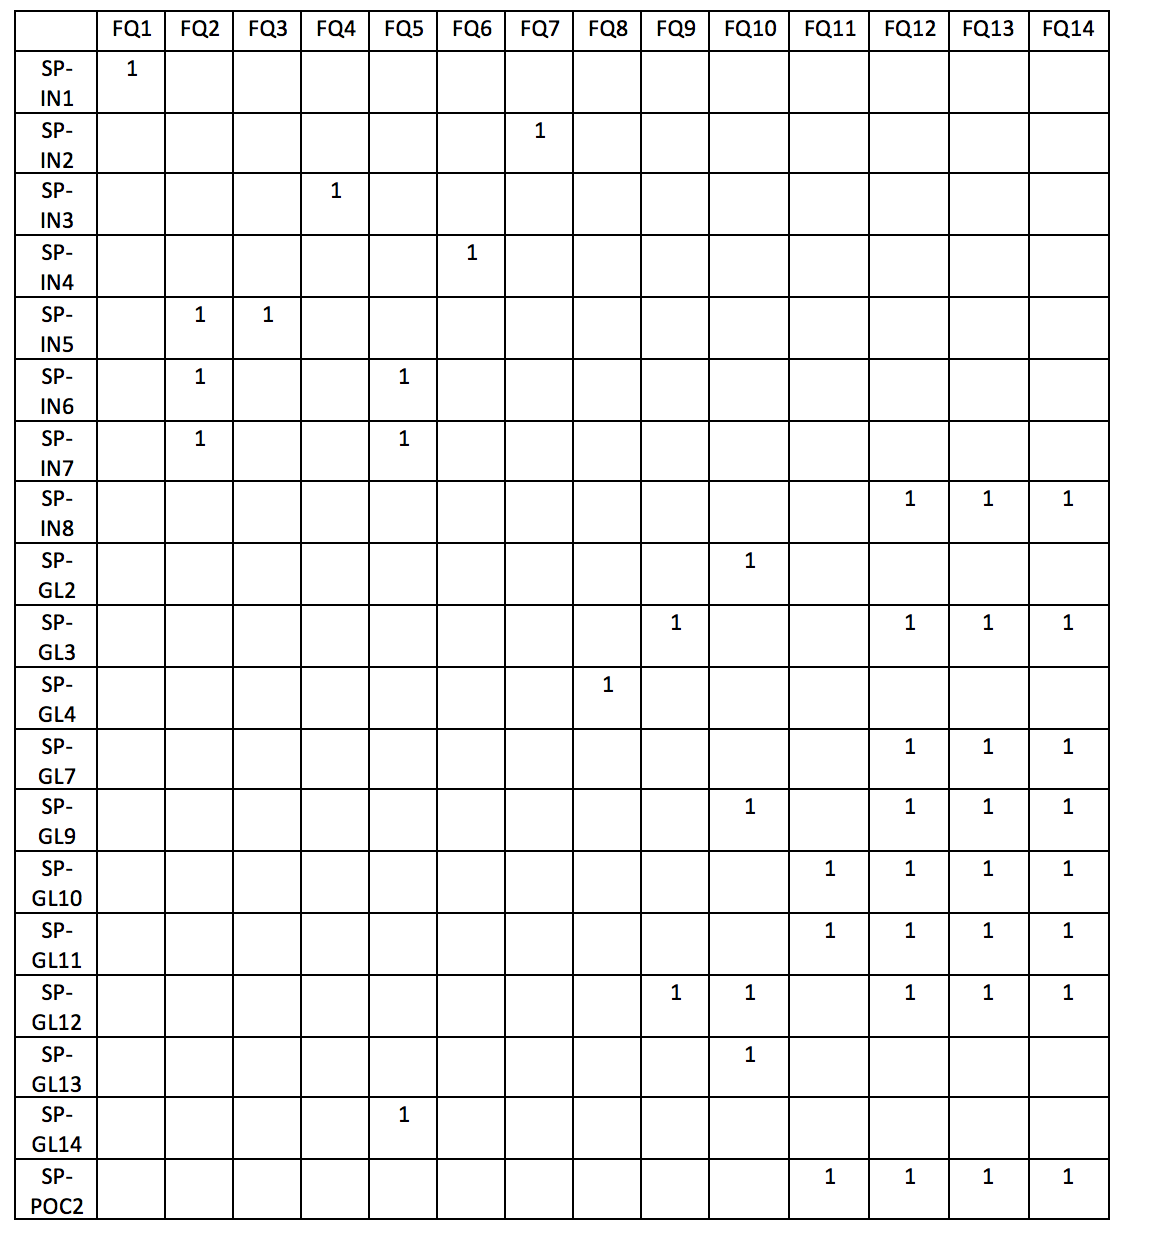
\includegraphics[width=0.9\textwidth]{traceq.png}
\caption{{\color{red}Traceability Testing Matrix respect to requirements}}
\label{FigUH}
\end{figure}		

\section{Trace to Modules}	
refer to the table in the end of the document.	
\begin{figure}[h]
\centering
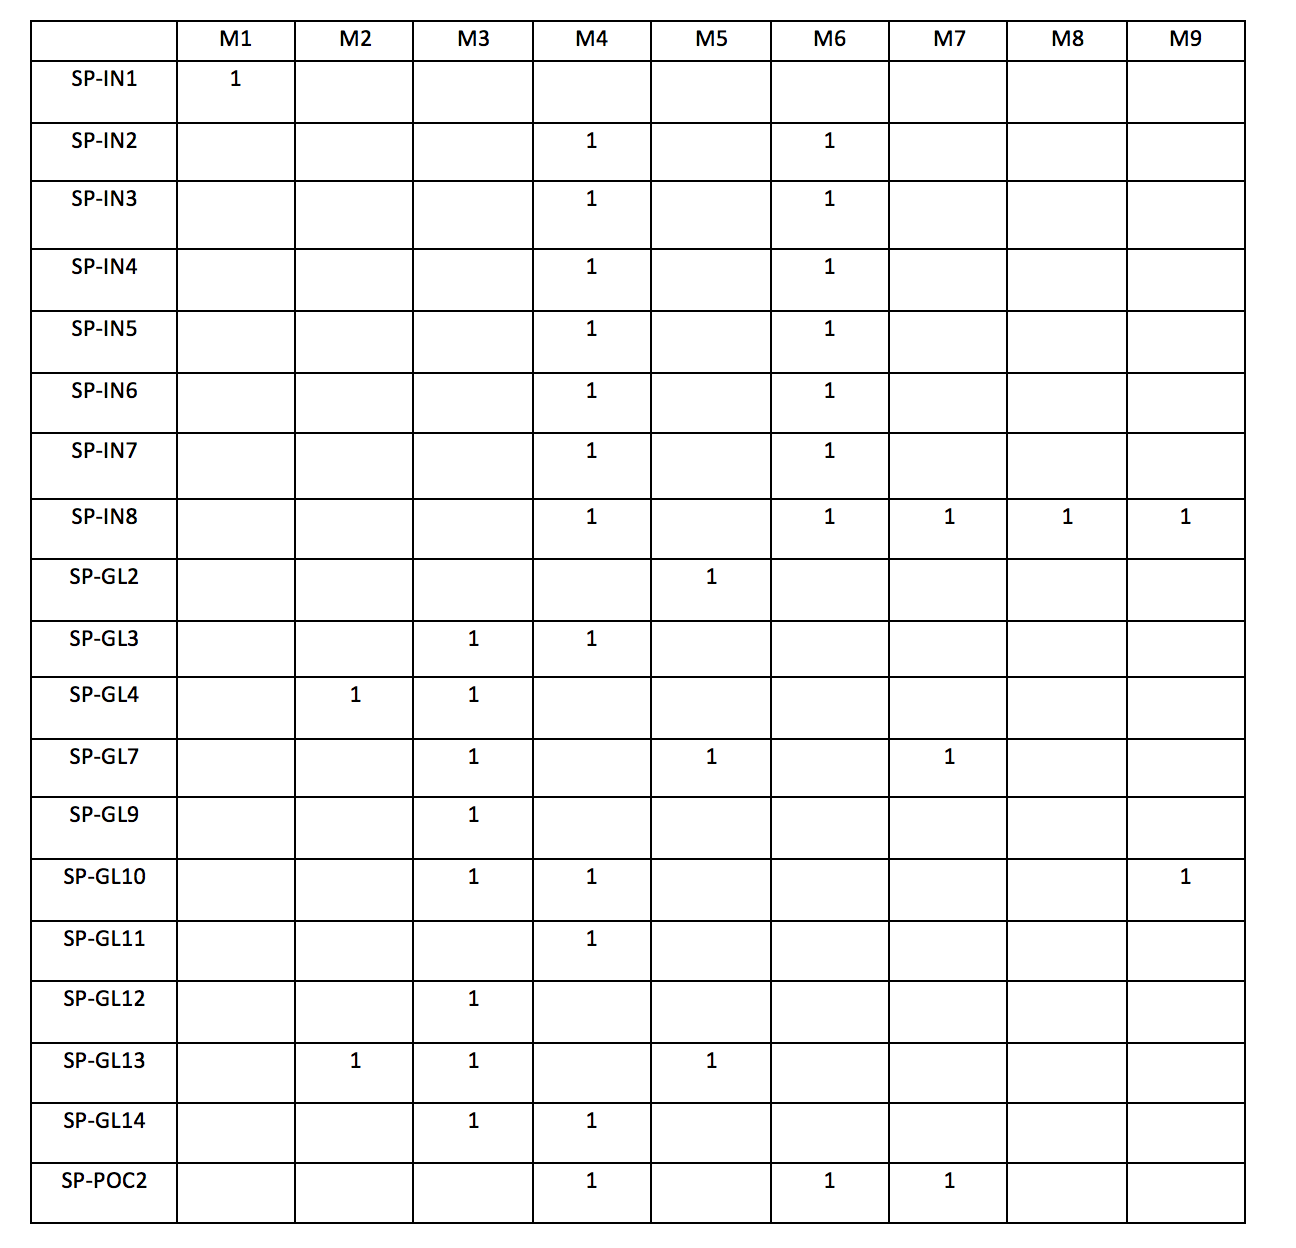
\includegraphics[width=0.9\textwidth]{tracem.png}
\caption{{\color{red}Traceability Testing Matrix respect to modules}}
\label{FigUH}
\end{figure}	
\section{Code Coverage Metrics}
Mocha testing shall test 80\% of the functions including edge cases. The rest of the codes are mostly in HTML and the purpose of HTML is to connect the system to the website and create the layout. As a result, it is not that meaningful to test and HTML is hard to be tested. Thus, basically, we manually test the layout part. In conclusion, the test coverage shall be above 75\%.
\bibliographystyle{plainnat}

\bibliography{SRS}

\end{document}